\documentclass{standalone}
\usepackage{tikz}
\usetikzlibrary{patterns, positioning}
\usepackage[sfdefault]{ClearSans} %% option 'sfdefault' activates Clear Sans as the default text font
\usepackage[T1]{fontenc}

\begin{document}
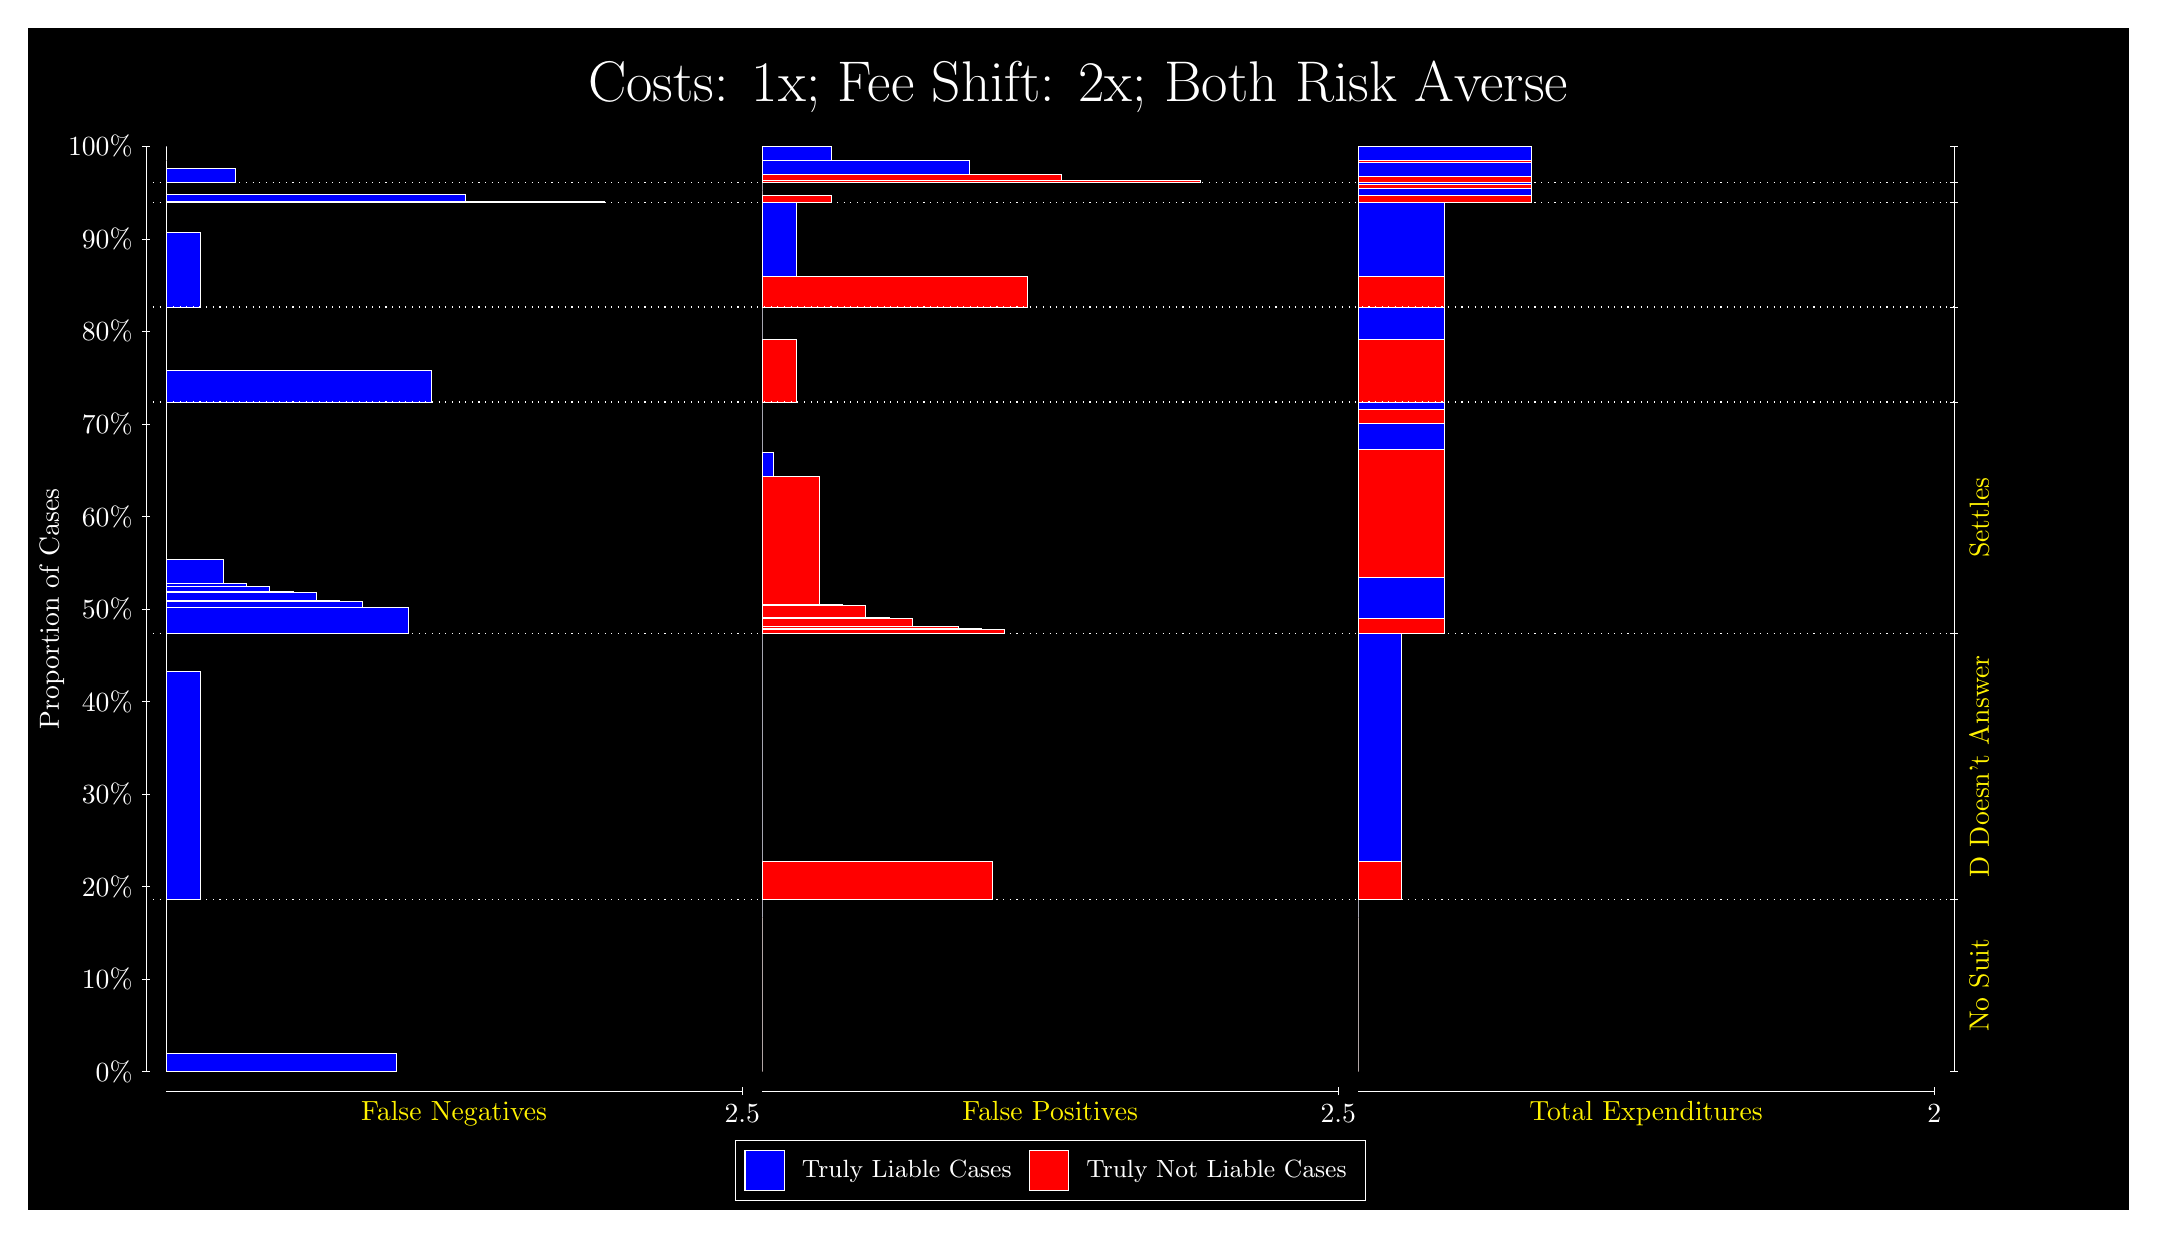
\begin{tikzpicture}
\draw[fill=black] (0,0) rectangle (26.667,15);
\draw[text=white] (0,13.5) rectangle (26.667,15) node[midway] {\huge Costs: 1x; Fee Shift: 2x; Both Risk Averse};
\draw[white, very thin] (1.5,1.75) -- (1.5,13.5);
\node[rotate=90, text=white, anchor=center] at (0.3, 7.625) {Proportion of Cases};
\draw[white, very thin] (1.45,1.75) -- (1.55,1.75);
\node[text=white, anchor=east] at (1.45, 1.75) {0\%};
\draw[white, very thin] (1.45,2.925) -- (1.55,2.925);
\node[text=white, anchor=east] at (1.45, 2.925) {10\%};
\draw[white, very thin] (1.45,4.1) -- (1.55,4.1);
\node[text=white, anchor=east] at (1.45, 4.1) {20\%};
\draw[white, very thin] (1.45,5.275) -- (1.55,5.275);
\node[text=white, anchor=east] at (1.45, 5.275) {30\%};
\draw[white, very thin] (1.45,6.45) -- (1.55,6.45);
\node[text=white, anchor=east] at (1.45, 6.45) {40\%};
\draw[white, very thin] (1.45,7.625) -- (1.55,7.625);
\node[text=white, anchor=east] at (1.45, 7.625) {50\%};
\draw[white, very thin] (1.45,8.8) -- (1.55,8.8);
\node[text=white, anchor=east] at (1.45, 8.8) {60\%};
\draw[white, very thin] (1.45,9.975) -- (1.55,9.975);
\node[text=white, anchor=east] at (1.45, 9.975) {70\%};
\draw[white, very thin] (1.45,11.15) -- (1.55,11.15);
\node[text=white, anchor=east] at (1.45, 11.15) {80\%};
\draw[white, very thin] (1.45,12.325) -- (1.55,12.325);
\node[text=white, anchor=east] at (1.45, 12.325) {90\%};
\draw[white, very thin] (1.45,13.5) -- (1.55,13.5);
\node[text=white, anchor=east] at (1.45, 13.5) {100\%};

\draw[white, very thin] (24.457,1.75) -- (24.457,13.5);
\draw[white, very thin] (24.407,1.75) -- (24.507,1.75);
\node[anchor=west] at (24.407, 1.75) {};
\draw[white, very thin] (24.407,3.9363) -- (24.507,3.9363);
\node[anchor=west] at (24.407, 3.9363) {};
\draw[white, very thin] (24.407,7.3115) -- (24.507,7.3115);
\node[anchor=west] at (24.407, 7.3115) {};
\draw[white, very thin] (24.407,10.253) -- (24.507,10.253);
\node[anchor=west] at (24.407, 10.253) {};
\draw[white, very thin] (24.407,11.46) -- (24.507,11.46);
\node[anchor=west] at (24.407, 11.46) {};
\draw[white, very thin] (24.407,12.788) -- (24.507,12.788);
\node[anchor=west] at (24.407, 12.788) {};
\draw[white, very thin] (24.407,13.044) -- (24.507,13.044);
\node[anchor=west] at (24.407, 13.044) {};
\draw[white, very thin] (24.407,13.5) -- (24.507,13.5);
\node[anchor=west] at (24.407, 13.5) {};

\draw[white, very thin, fill=blue] (1.75,1.75) rectangle (4.6775,1.98);
\draw[white, very thin, fill=red] (1.75,1.98) rectangle (1.75,3.9363);
\draw[white, very thin, fill=blue] (1.75,3.9363) rectangle (2.1891,6.831);
\draw[white, very thin, fill=red] (1.75,6.831) rectangle (1.75,7.3115);
\draw[white, very thin, fill=blue] (1.75,7.3115) rectangle (4.8239,7.6424);
\draw[white, very thin, fill=blue] (1.75,7.6424) rectangle (4.5312,7.6513);
\draw[white, very thin, fill=blue] (1.75,7.6513) rectangle (4.2384,7.7281);
\draw[white, very thin, fill=blue] (1.75,7.7281) rectangle (3.9457,7.737);
\draw[white, very thin, fill=blue] (1.75,7.737) rectangle (3.6529,7.8416);
\draw[white, very thin, fill=blue] (1.75,7.8416) rectangle (3.3602,7.8547);
\draw[white, very thin, fill=blue] (1.75,7.8547) rectangle (3.0674,7.908);
\draw[white, very thin, fill=blue] (1.75,7.908) rectangle (2.7746,7.9457);
\draw[white, very thin, fill=blue] (1.75,7.9457) rectangle (2.4819,8.2559);
\draw[white, very thin, fill=red] (1.75,8.2559) rectangle (1.75,10.253);
\draw[white, very thin, fill=blue] (1.75,10.253) rectangle (5.1167,10.66);
\draw[white, very thin, fill=red] (1.75,10.66) rectangle (1.75,11.46);
\draw[white, very thin, fill=blue] (1.75,11.46) rectangle (2.1891,12.403);
\draw[white, very thin, fill=red] (1.75,12.403) rectangle (1.75,12.788);
\draw[white, very thin, fill=blue] (1.75,12.788) rectangle (7.3123,12.808);
\draw[white, very thin, fill=blue] (1.75,12.808) rectangle (5.5558,12.891);
\draw[white, very thin, fill=red] (1.75,12.891) rectangle (1.75,13.044);
\draw[white, very thin, fill=blue] (1.75,13.044) rectangle (2.6283,13.217);
\draw[white, very thin, fill=red] (1.75,13.217) rectangle (1.75,13.321);
\draw[white, very thin, fill=blue] (1.75,13.321) rectangle (1.75,13.5);
\draw[white, very thin, fill=red] (9.3189,1.75) rectangle (9.3189,3.7063);
\draw[white, very thin, fill=blue] (9.3189,3.7063) rectangle (9.3189,3.9363);
\draw[white, very thin, fill=red] (9.3189,3.9363) rectangle (12.246,4.4167);
\draw[white, very thin, fill=blue] (9.3189,4.4167) rectangle (9.3189,7.3115);
\draw[white, very thin, fill=red] (9.3189,7.3115) rectangle (12.393,7.3617);
\draw[white, very thin, fill=red] (9.3189,7.3617) rectangle (12.1,7.3787);
\draw[white, very thin, fill=red] (9.3189,7.3787) rectangle (11.807,7.4029);
\draw[white, very thin, fill=red] (9.3189,7.4029) rectangle (11.515,7.4088);
\draw[white, very thin, fill=red] (9.3189,7.4088) rectangle (11.222,7.5063);
\draw[white, very thin, fill=red] (9.3189,7.5063) rectangle (10.929,7.5151);
\draw[white, very thin, fill=red] (9.3189,7.5151) rectangle (10.636,7.6741);
\draw[white, very thin, fill=red] (9.3189,7.6741) rectangle (10.344,7.6829);
\draw[white, very thin, fill=red] (9.3189,7.6829) rectangle (10.051,9.308);
\draw[white, very thin, fill=blue] (9.3189,9.308) rectangle (9.4652,9.6183);
\draw[white, very thin, fill=blue] (9.3189,9.6183) rectangle (9.3189,10.253);
\draw[white, very thin, fill=red] (9.3189,10.253) rectangle (9.758,11.052);
\draw[white, very thin, fill=blue] (9.3189,11.052) rectangle (9.3189,11.46);
\draw[white, very thin, fill=red] (9.3189,11.46) rectangle (12.686,11.845);
\draw[white, very thin, fill=blue] (9.3189,11.845) rectangle (9.758,12.788);
\draw[white, very thin, fill=red] (9.3189,12.788) rectangle (10.197,12.884);
\draw[white, very thin, fill=red] (9.3189,12.884) rectangle (9.3189,12.941);
\draw[white, very thin, fill=blue] (9.3189,12.941) rectangle (9.3189,13.044);
\draw[white, very thin, fill=red] (9.3189,13.044) rectangle (14.881,13.073);
\draw[white, very thin, fill=red] (9.3189,13.073) rectangle (13.125,13.148);
\draw[white, very thin, fill=blue] (9.3189,13.148) rectangle (11.954,13.327);
\draw[white, very thin, fill=blue] (9.3189,13.327) rectangle (10.197,13.5);
\draw[white, very thin, fill=red] (16.888,1.75) rectangle (16.888,3.7063);
\draw[white, very thin, fill=blue] (16.888,3.7063) rectangle (16.888,3.9363);
\draw[white, very thin, fill=red] (16.888,3.9363) rectangle (17.437,4.4167);
\draw[white, very thin, fill=blue] (16.888,4.4167) rectangle (17.437,7.3115);
\draw[white, very thin, fill=red] (16.888,7.3115) rectangle (17.986,7.5063);
\draw[white, very thin, fill=blue] (16.888,7.5063) rectangle (17.986,8.0252);
\draw[white, very thin, fill=red] (16.888,8.0252) rectangle (17.986,9.6503);
\draw[white, very thin, fill=blue] (16.888,9.6503) rectangle (17.986,9.9813);
\draw[white, very thin, fill=red] (16.888,9.9813) rectangle (17.986,10.158);
\draw[white, very thin, fill=blue] (16.888,10.158) rectangle (17.986,10.253);
\draw[white, very thin, fill=red] (16.888,10.253) rectangle (17.986,11.052);
\draw[white, very thin, fill=blue] (16.888,11.052) rectangle (17.986,11.46);
\draw[white, very thin, fill=red] (16.888,11.46) rectangle (17.986,11.845);
\draw[white, very thin, fill=blue] (16.888,11.845) rectangle (17.986,12.788);
\draw[white, very thin, fill=red] (16.888,12.788) rectangle (19.083,12.884);
\draw[white, very thin, fill=blue] (16.888,12.884) rectangle (19.083,12.967);
\draw[white, very thin, fill=red] (16.888,12.967) rectangle (19.083,13.024);
\draw[white, very thin, fill=blue] (16.888,13.024) rectangle (19.083,13.044);
\draw[white, very thin, fill=red] (16.888,13.044) rectangle (19.083,13.119);
\draw[white, very thin, fill=blue] (16.888,13.119) rectangle (19.083,13.293);
\draw[white, very thin, fill=red] (16.888,13.293) rectangle (19.083,13.321);
\draw[white, very thin, fill=blue] (16.888,13.321) rectangle (19.083,13.5);
\draw[white, dotted] (1.5,3.9363) -- (24.457,3.9363);
\draw[white, dotted] (1.5,7.3115) -- (24.457,7.3115);
\draw[white, dotted] (1.5,10.253) -- (24.457,10.253);
\draw[white, dotted] (1.5,11.46) -- (24.457,11.46);
\draw[white, dotted] (1.5,12.788) -- (24.457,12.788);
\draw[white, dotted] (1.5,13.044) -- (24.457,13.044);
\draw[white, very thin] (1.75,1.5) -- (9.0689,1.5);
\node[text=yellow, anchor=north] at (5.4094, 1.5) {False Negatives};
\draw[white, very thin] (9.0689,1.45) -- (9.0689,1.55);
\node[text=white, anchor=north] at (9.0689, 1.45) {2.5};

\draw[white, very thin] (9.3189,1.5) -- (16.638,1.5);
\node[text=yellow, anchor=north] at (12.978, 1.5) {False Positives};
\draw[white, very thin] (16.638,1.45) -- (16.638,1.55);
\node[text=white, anchor=north] at (16.638, 1.45) {2.5};

\draw[white, very thin] (16.888,1.5) -- (24.207,1.5);
\node[text=yellow, anchor=north] at (20.547, 1.5) {Total Expenditures};
\draw[white, very thin] (24.207,1.45) -- (24.207,1.55);
\node[text=white, anchor=north] at (24.207, 1.45) {2};

\node[text=yellow, centered, rotate=90] at (24.777, 2.8432) {No Suit};
\node[text=yellow, centered, rotate=90] at (24.777, 5.6239) {D Doesn't Answer};
\node[text=yellow, centered, rotate=90] at (24.777, 8.782) {Settles};





\draw (12.978300999999998,1.5) node[draw=none] (baseCoordinate) {};
\begin{scope}[align=center]
        \matrix[scale=0.5, draw=white, below=0.5cm of baseCoordinate, nodes={draw}, column sep=0.1cm]{
            \node[rectangle, draw, minimum width=0.5cm, minimum height=0.5cm, fill=blue] {}; &
            \node[draw=none, font=\small, text=white] (B) {Truly Liable Cases}; &
            \node[rectangle, draw, minimum width=0.5cm, minimum height=0.5cm, fill=red] {}; &
            \node[draw=none, font=\small, text=white] (B) {Truly Not Liable Cases}; \\
            };
\end{scope}

\end{tikzpicture}
\end{document}